\index{bed leveling}
\section{Bed Leveling}
Make sure you take the time to go through the following procedure to help ensure that your prints are consistent and trouble free. Make sure to first read the instructions for using the Printrun software. Connect to the printer as described in the Printrun software section. Once \texttt{Pronterface} is connected to the printer use the homing buttons to home the X and Y axis. \color{red}{Do not use the \texttt{HomeZ button}until after the \texttt{Z axis End stop} has been adjusted. Make sure that the red shipping clamps on the Z axis smooth rods have been removed before continuing.}

\index{z axis}
\subsection{Lowering the Z Axis}
Once connected to the TAZ 3D printer in Pronterface, Use the \texttt{-Z 1 button} to move the Z axis down in \texttt{1mm} increments. Move the Z axis down towards the bed by 5mm at first. While the Z axis is moving down pay attention to the Z axis movement and sound. The Z axis stepper motors should be moving in unison. If you notice a grinding sound stop and, before proceeding, make sure that the Z axis looks level in relation to the body of the TAZ 3D printer. Once you have confirmed smooth movement of the Z axis, use the \texttt{-Z 10 button} to move the Z axis down in 10mm increments. \textcolor{red}{Commands sent in Pronterface will stack, so multiple movement button presses can potentially be harmful and cannot be stopped without powering down the 3D printer.} Keep an eye on the nozzle for the hot end. As it approaches the surface of the bed use the \texttt{-Z 1 button} to continue lowering the Z axis into position. Stop lowering the Z axis once the Z axis has been lowered to within 4 inches(100mm) of the bed.

\subsection{Verify Z Axis Leveling}
With the Z axis lowered near the bed, use the included \texttt{150mm ruler} to measure the distance from the bottom of the \texttt{X axis} smooth rod and the top surface of the \texttt{Y axis} aluminum bed plate on the left side.
\begin{figure}[H]
\centering
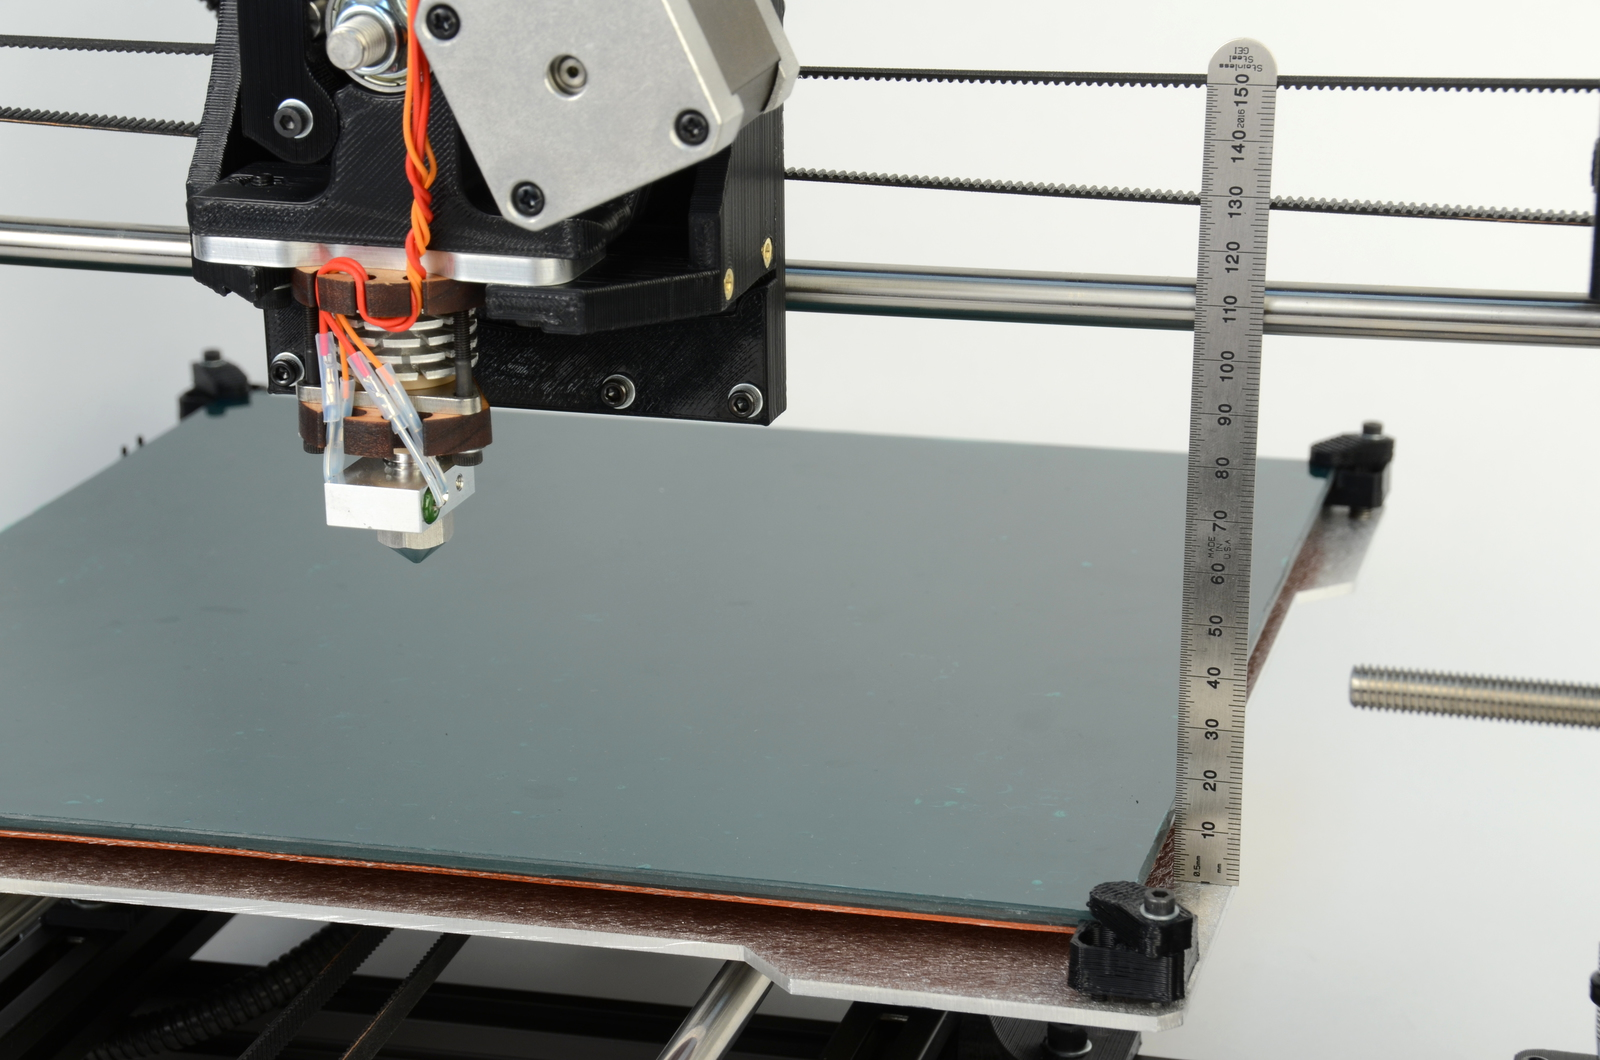
\includegraphics[keepaspectratio=true,angle=0,height=0.4\textheight,width=1.0\textwidth]{X-Y_axes_leveling_check.JPG}
\caption{Verifying the X and Y axis are square}
\label{fig:X-Y_axes_leveling_check}
\end{figure} 
Compare the distance measurement from the left side to the measurement on the right side. The distance measurement should be the same. If not, in Pronterface use the \texttt{Motors off} button to turn off the stepper motors on the TAZ 3D printer. Manually, by hand, turn the threaded rod on one side of the printer to raise or lower that side to match the measurement on the other side. If the Z axis has been adjusted measure again to confirm that the left and right side of the Z axis are level in relation to the Y axis aluminum plate.

\subsection{Rough Adjustment of the Z Axis End Stop}
\index{end stop}
Before using the \texttt{home Z} button or the \texttt{home all} button you will need to adjust the \texttt{Z axis endstop}.
\begin{figure}[p]
\centering
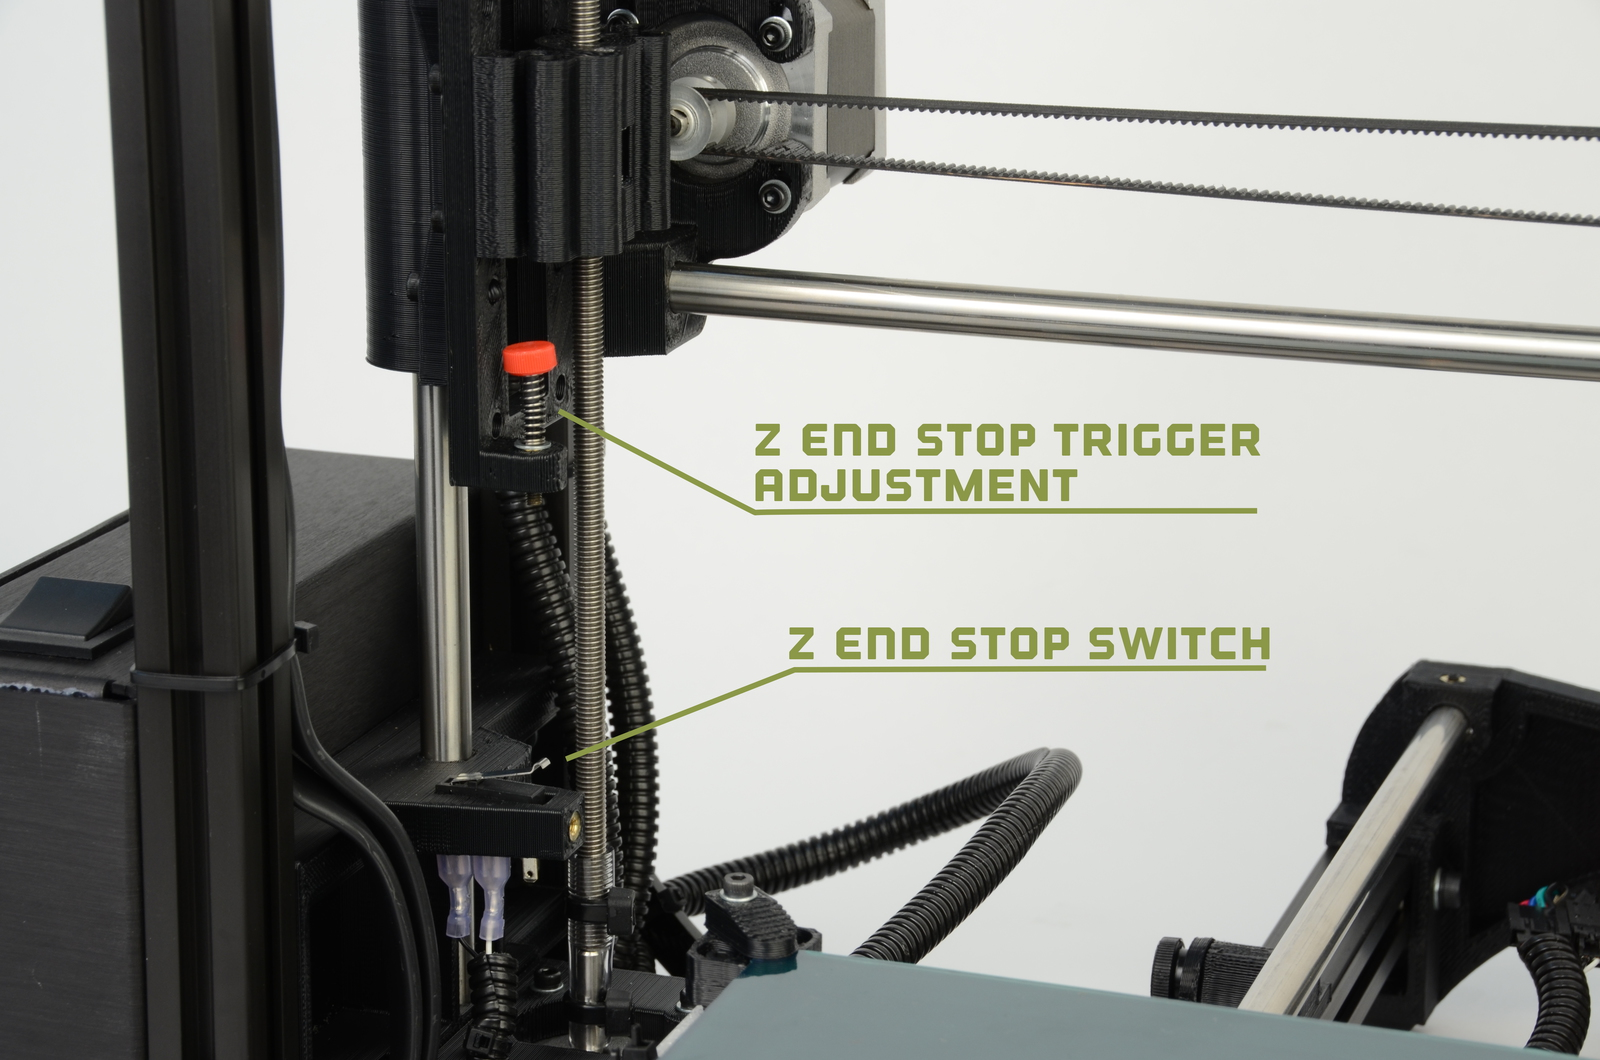
\includegraphics[keepaspectratio=true,angle=0,height=0.4\textheight,width=1.0\textwidth]{Z_end_stop_trigger.JPG}
\caption{Z end stop trigger}
\label{fig:Z_end_stop_trigger}
\end{figure}
Rotate the \texttt{Z axis end stop trigger} clockwise to lower the bottom of the screw closer to the Z axis end stop. Once lowered by approximately 1cm, press the \texttt{HomeZ button} to home the Z axis. The hot end will approach the heated bed and will likely stop around a centimeter above the surface of the heated bed.

\subsection{Fine Adjustment of the Z Axis End Stop}
Adjust the \texttt{Z axis end stop trigger} by rotating the screw counter-clockwise to raise the tip of the screw. Raise the screw by roughly the same amount of the distance between the nozzle tip and the print surface. Press the \texttt{Home Z}button to home the Z axis. The tip of the nozzle should now be very close to the surface of the bed.

\subsection{Leveling the Print Bed}
Slide a thin piece of paper underneath the nozzle in the front left corner of the bed. Adjust the z axis end stop and home the Z axis until the tip of the nozzle applies a firm pressure on the paper. Try to slide the paper from underneath the the tip of the nozzle. It should not tear, but some resistance should be felt. Move the hot end nozzle tip over to the far side of the X axis by using the \texttt{+X 100 button}. As the X axis carriage approaches the end of the X axis use the \texttt{+X 10 button} and finally the \texttt{+X 1 button}. Once the tip of the nozzle is near the front right corner of the bed slide the same piece of paper under the nozzle and home the Z axis. To raise or lower the front right corner of the bed adjust the third screw from the left. Do not adjust the middle screw. Adjust the front right corner of the bed until the amount of tension felt when moving the piece of paper under the nozzle feels the same as the tension felt when doing the same thing on the front left corner. Repeat the same process using the \texttt{+Y button} to move the heated bed to place the nozzle on the rear right corner of the bed. Adjust the height of the bed using the same procedure as outlined above. Finally, move the X axis carriage over to the rear left corner of the bed and perform the same leveling procedure to adjust the last corner. The bed should now be almost perfectly level. We will check this in a later section. Use the controls in Printrun to raise the Z axis up 20mm, and move the X axis carriage over to the center of the X axis.

\section{Set Temperature}
\index{temperature}
%Make sure to first read the instructions for using the Printrun software. Connect to the printer as described in the Printrun software section
%%% XXX pageref going to \label not \section (page \pageref{Installing Printrun}).
Set the hot end and print surface for ABS or PLA plastic and turn both on. The temperature settings for ABS should be set at \texttt{230°C} for the hot end and \texttt{85°C} for print surface; for PLA they should be set at \texttt{185°C} for the hot end and \texttt{55°C} for print surface. Click the \texttt{Motors Off} button.
\glossary{Idler}{Refers to parts using a bearing (usually a 608ZZ) to add tension in belts or to add pressure against a rolling surface.}
\section{Load Filament}
\index{filament}
\index{hot end}

Once the hot end is heated to the correct temperature you will now need to load the plastic filament into the extruder. Raise both the idler clip and the 2 screws adding tension to release the hinged idler. It can be loosened if necessary. If the extruder has a small section of filament already loaded, you will need to remove the filament once the extruder idler has been opened by gently pulling out the filament by hand once the hot end has reached the extrusion temperature of \texttt{230C}
(Fig. \ref{fig:extruder_idler_release}).
\begin{figure}[hbt]
\centering
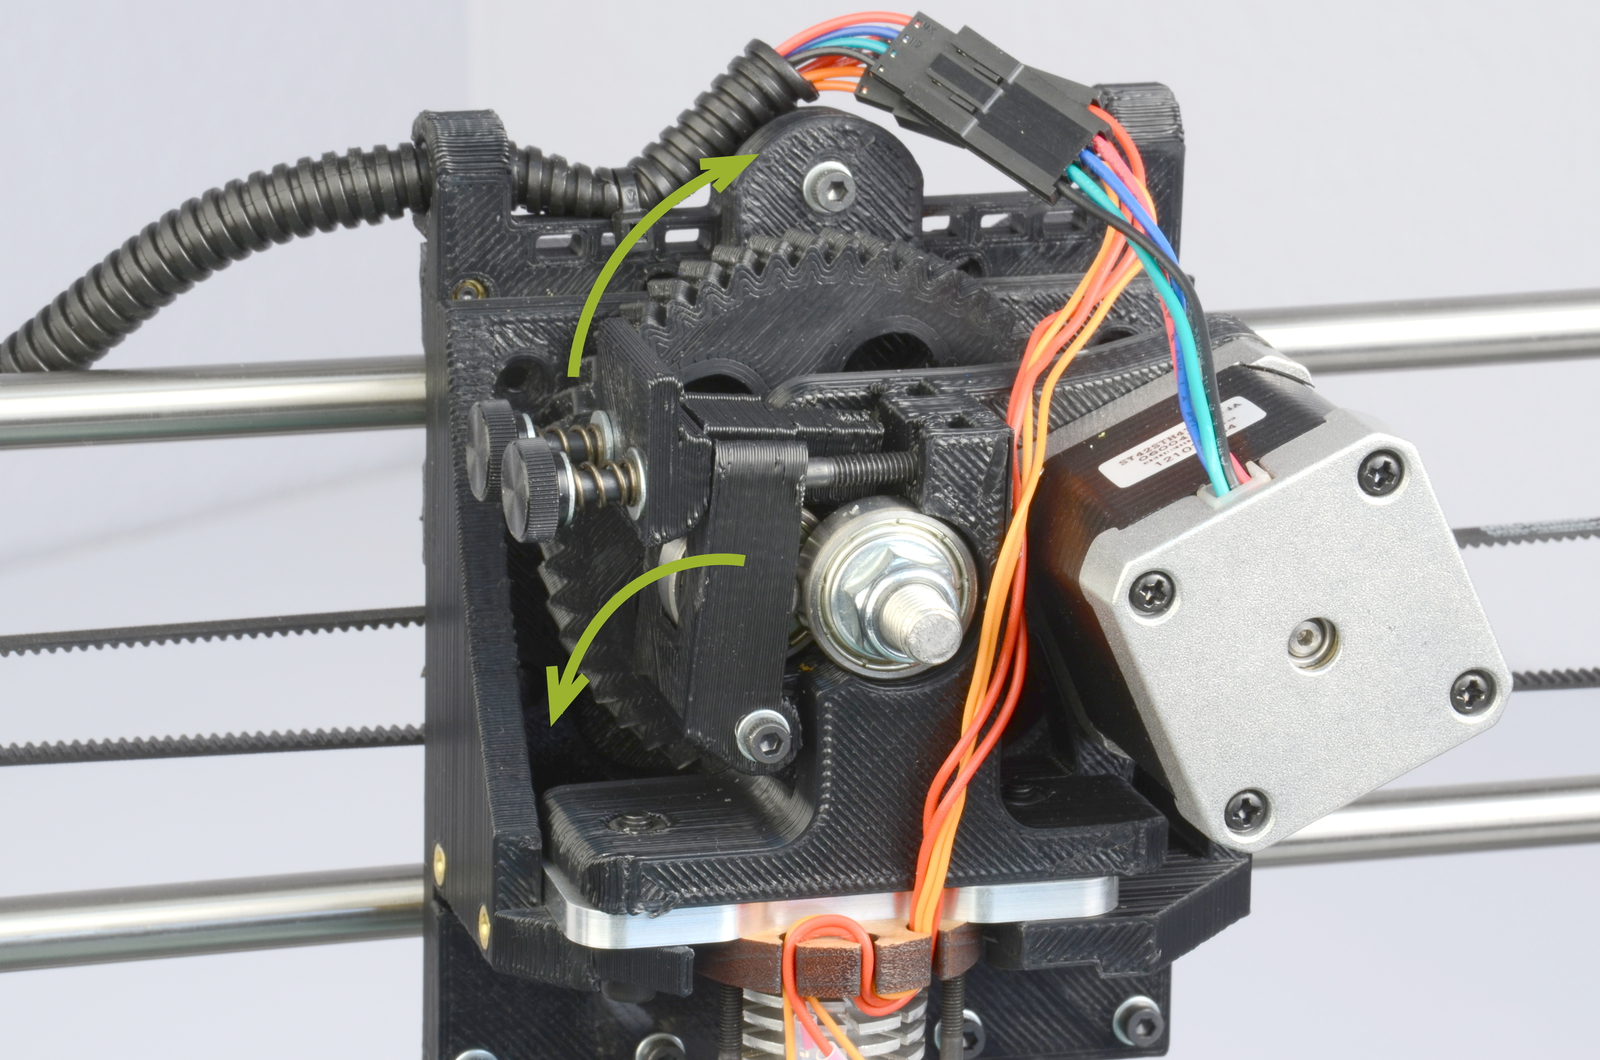
\includegraphics[keepaspectratio=true,angle=0,height=0.4\textheight,width=1.0\textwidth]{extruder_idler_release.JPG}
\caption{Extruder idler release}
\label{fig:extruder_idler_release}
\end{figure}
% update feed hole picture.
Gently squeeze both the idler screws and the plastic clip together and pull upwards to release the idler. The idler can be rotated downwards allowing access to the hobbed bolt and filament feed hole(Fig. \ref{fig:extruder_filament_slot}, page \pageref{fig:extruder_filament_slot}). Feed the end of the plastic filament into the filament feed hole
(Fig. \ref{fig:extruder_filament_slot}).
\begin{figure}[hbt]
\centering
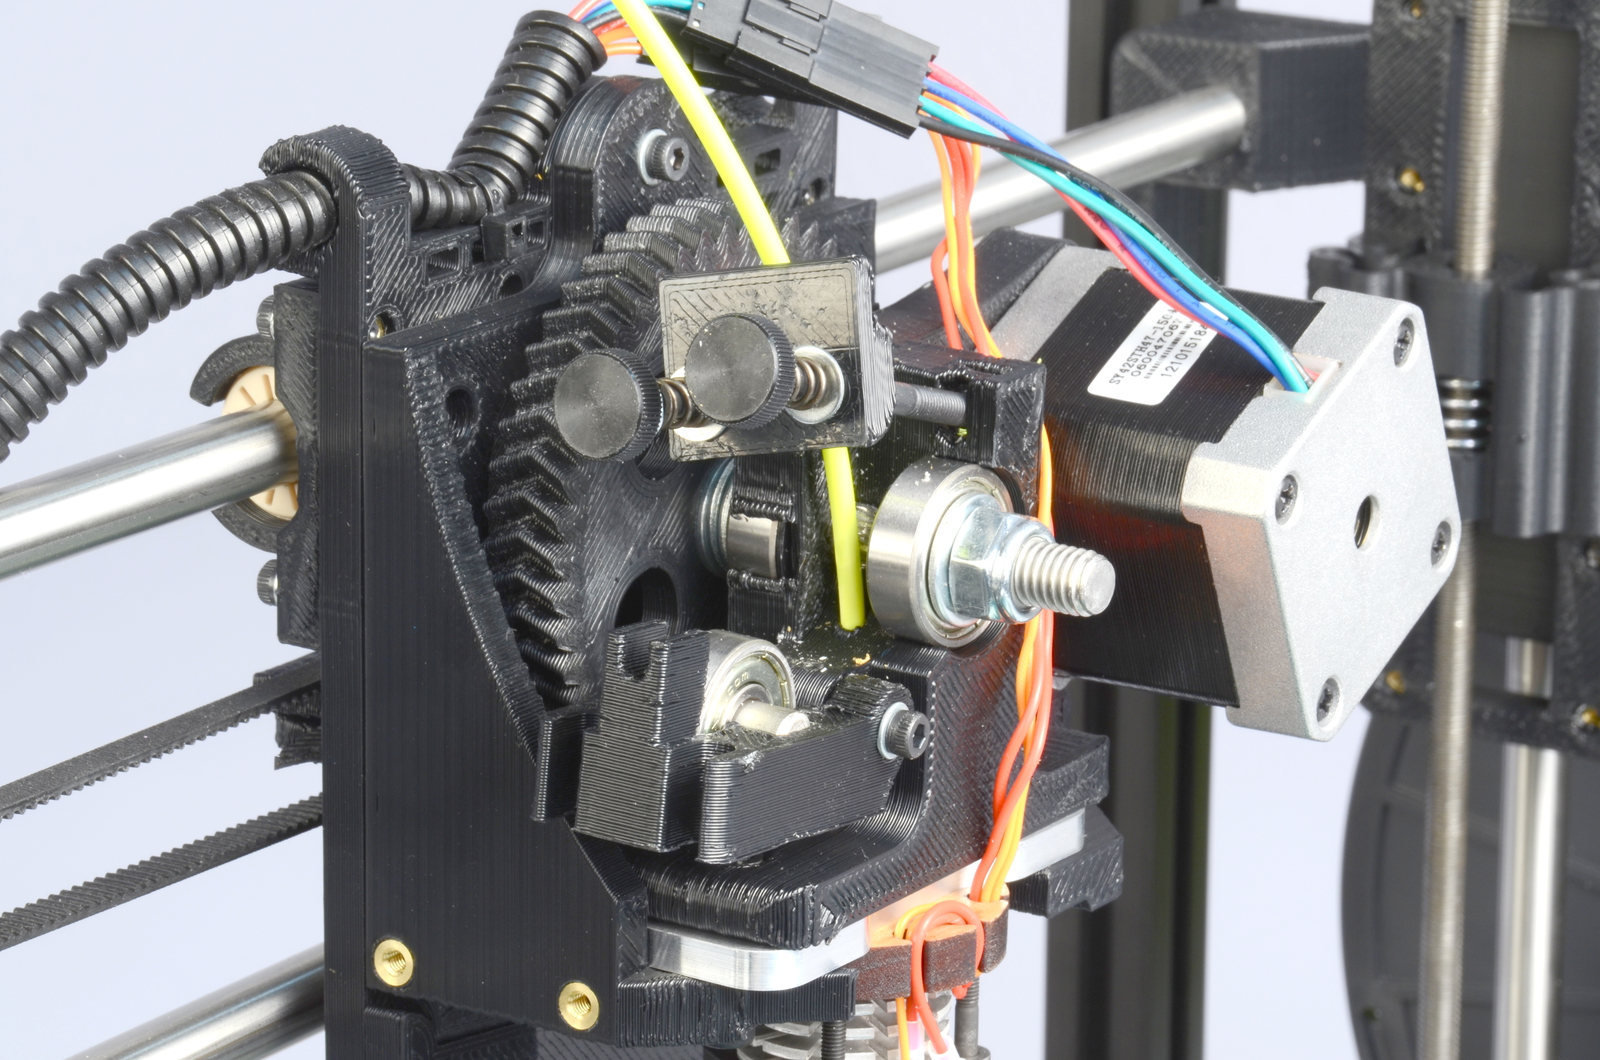
\includegraphics[keepaspectratio=true,angle=0,height=0.4\textheight,width=1.0\textwidth]{extruder_filament_slot.JPG}
\caption{Extruder filament slot}
\label{fig:extruder_filament_slot}
\end{figure}
Now you can push the filament through the extruder by slowly pushing the filament down into the hot end.

Once the filament extrudes a small amount out of the nozzle raise the idler and slide the two idler bolts and plate back into place. Tighten the two idler bolts if you previously loosened them. Tighten the two screws until they are finger tight, then tighten them slightly more. Now use the \texttt{Extrude} button in Printrun to test that the extruder is working properly. You may need to extrude 40-60mm of filament to fully prime the hot end. Adjust the tension on the two screws until you can reliable and repeatedly extrude roughly 40mm of filament.

\section{Home Printer}
Use the home buttons to home the X axis and then the Y axis. Next home the Z axis. When the Z axis is at home the nozzle tip should be sitting right against the glass
(Fig. \ref{fig:nozzle_height}, page \pageref{fig:nozzle_height}). The image to the right, in figure \ref{fig:nozzle_height}, is the correct nozzle height.
\begin{figure}[p]
\centering
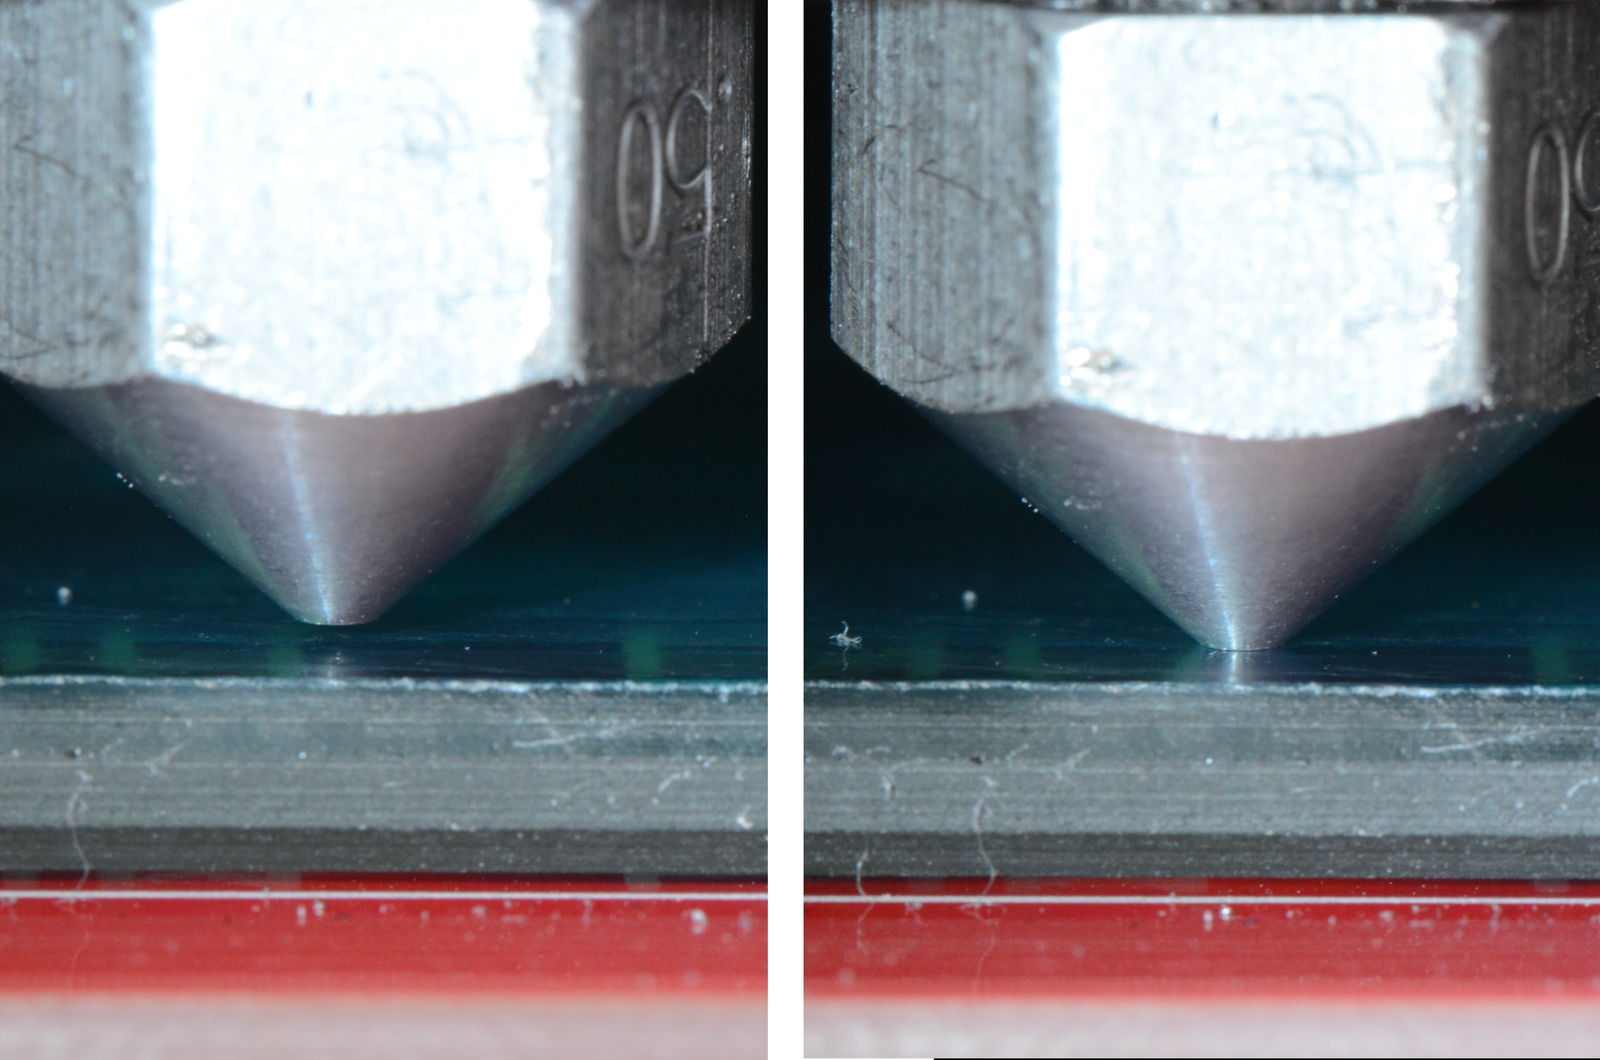
\includegraphics[keepaspectratio=true,angle=0,height=0.4\textheight,width=1.0\textwidth]{nozzle_height.jpg}
\caption{Nozzle height}
\label{fig:nozzle_height}
\end{figure}
\begin{figure}[p]
\centering
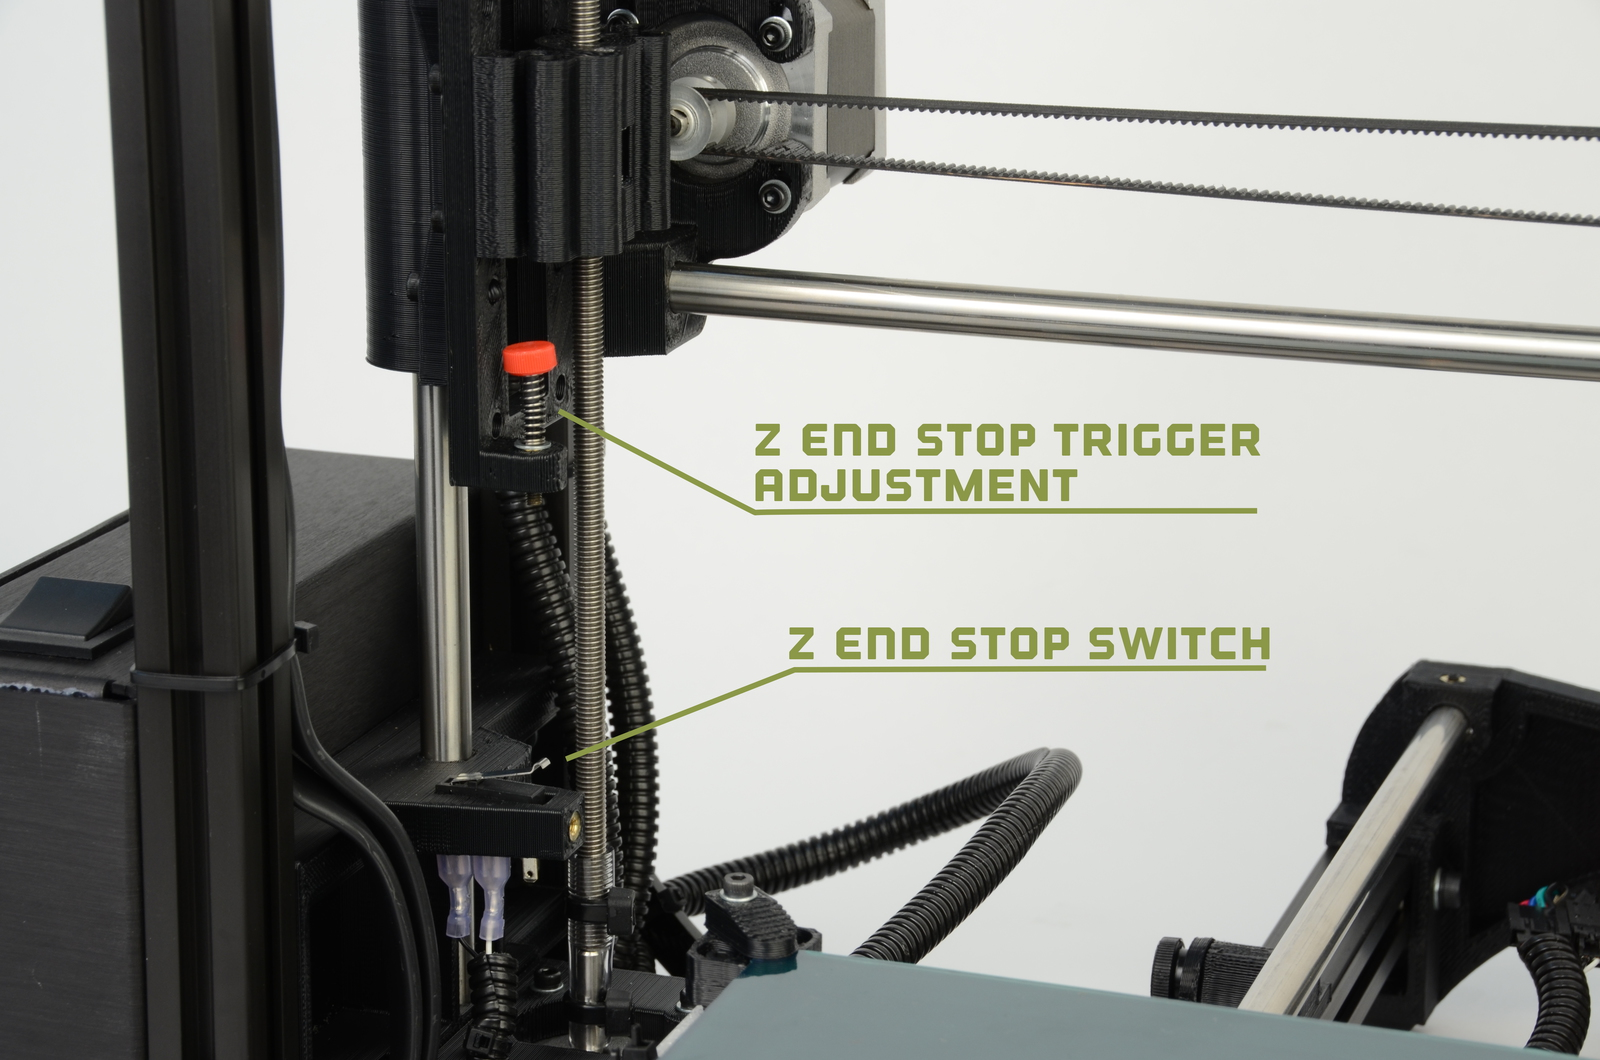
\includegraphics[keepaspectratio=true,angle=0,height=0.4\textheight,width=1.0\textwidth]{Z_end_stop_trigger.JPG}
\caption{Z end stop trigger}
\label{fig:Z_end_stop_trigger}
\end{figure}
The nozzle should not be pushing down on the print surface. To lower or raise the Z home height adjust the Z end stop trigger. The red end stop trigger is on the far left of the printer mounted on the X-axis motor mount.
(Fig. \ref{fig:Z_end_stop_trigger}, page \pageref{fig:Z_end_stop_trigger}).
The red end stop trigger can be lowered by turning clockwise and raised by turning counter-clockwise. Once you have homed the axes and the hot end and bed have reached the correct temperature it is time to print!

%fix image positioning, images for 5.3 get shoved underneath 5.4
\section{Z Print Height}
Load the \texttt{bedcalib.gco} file.
This file can be found at:
\texttt{http://download.lulzbot.com/TAZ/calibration/bed_level.gcode} once downloaded you your computer press the \texttt{Load file button}. Navigate through the file browser to the downloaded \texttt{bed_level.gcode} file.

The .gcode file should appear in the Printrun G-Code viewer. Press the \texttt{Print} button to begin the print. When the print starts make sure the first layer is not printing too close or too far from the print bed. Note 
Figure \ref{fig:1st_layer_adhesion}, page \pageref{fig:1st_layer_adhesion},
\begin{figure}[hbt]
\centering
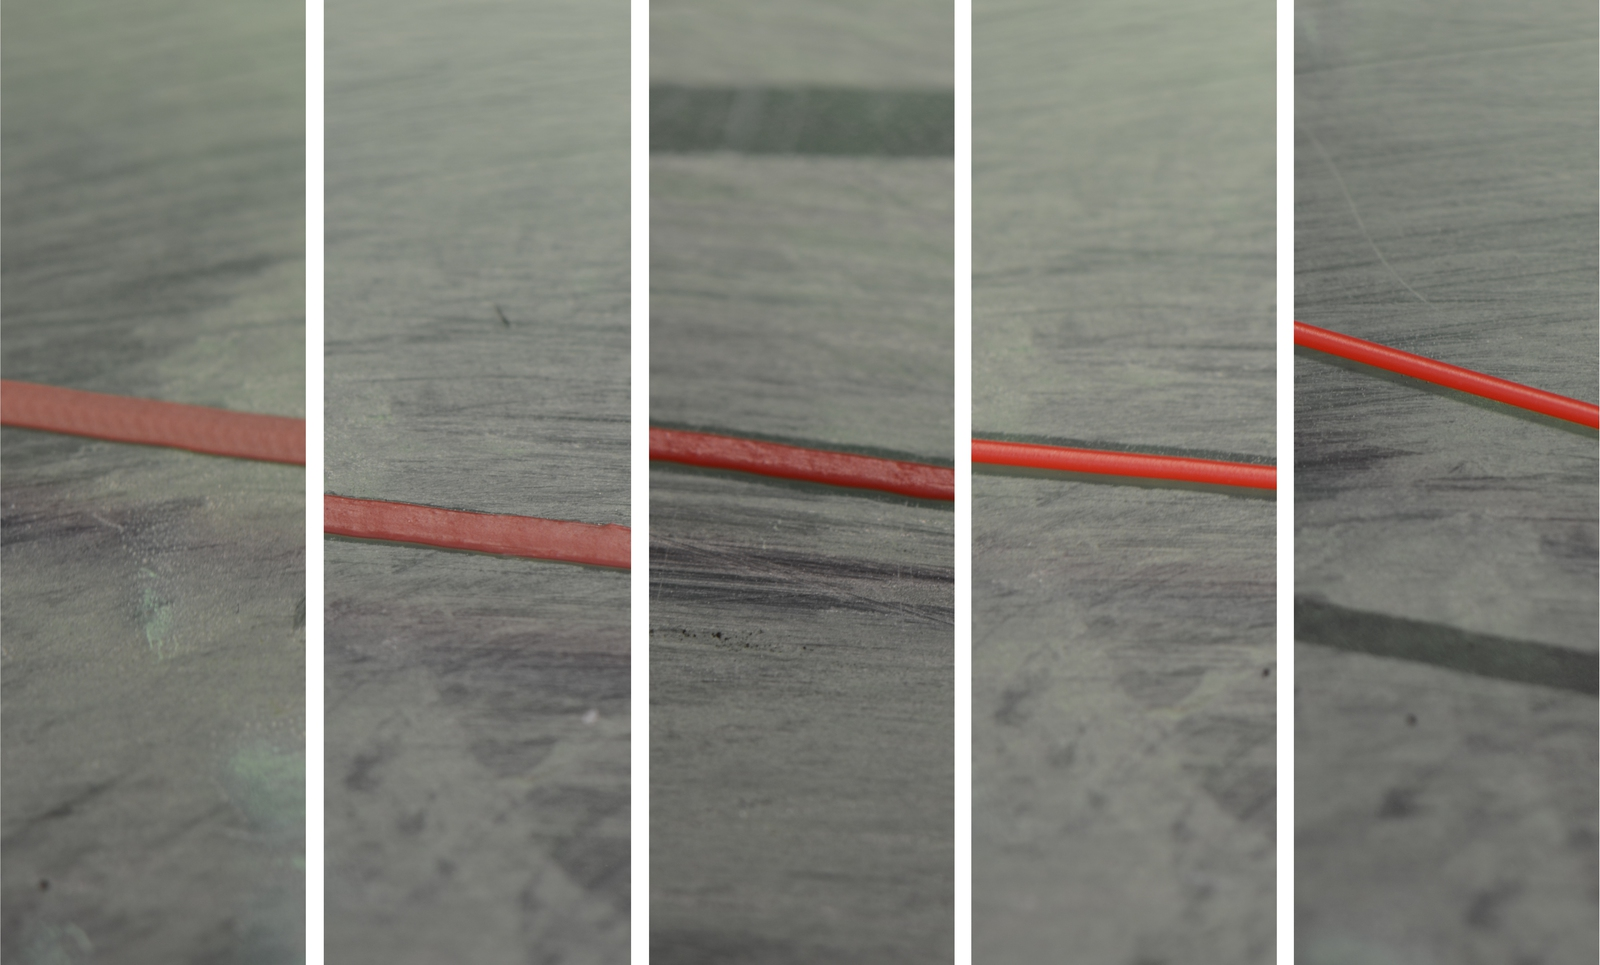
\includegraphics[keepaspectratio=true,angle=0,height=0.4\textheight,width=1.0\textwidth]{1st_layer_adhesion.jpg}
\caption{First layer adhesion}
\label{fig:1st_layer_adhesion}
\end{figure}
as an example of a good first layer adhesion. From left to right: very low, low, \emph{perfect,} high, very high. If the first layer is too high or low you can pause the print by pressing the \texttt{Pause} button. Adjust the Z end stop trigger. After making adjustments remove any printed material off the bed and home the axes and press \texttt{Restart} to restart the print. Measure the extrusion width, ideally the width would be the same in all areas of the bed. You would raise/lower a corner to minimize/increase the extrusion width to match the others. Once they are all consistent, the bed is level.

\section{Your First Print!}
Load the \texttt{octopus.gcode} file.
This file can be found at:
\texttt{http://download.lulzbot.com/TAZ/novelties/octopus.gcode}. Load the file in Pronterface, bring the hot end \texttt{(230C ABS/185C PLA))} and the heated bed \texttt{(85C ABS/60C PLA)} up to printing temperature. Once the printer is at the appropriate temperature, press the \texttt{Print} button to begin the print.

\section{Remove Part}
After the part is finished printing, the heated bed will automatically cool down to \texttt{60°C}. If you are printing PLA you will need to turn the heated bed off. Once the bed cools you can you pop the finished part off of the printed surface. To remove the printed part, use the clam knife included in your printer kit. Leather gloves are suggested to protect your hands from the clam knife blade. It is also safe practice to not place your hand behind the direction you are pushing the clam knife. Using the side of the clam knife blade pry up one side of the printed part. If your part is large you may need to pry at multiple points to pop the part off of the print surface. When removing parts take caution to not damage the PET film. If the film is cut or ripped it will peel from the glass and need to be replaced. Make sure to reset the heated bed to the correct temperature and allow it to heat up to the needed temperature before starting the next print.

